\documentclass[12pt, letterpaper]{report}
\usepackage{graphicx}
\usepackage{hyperref}
\usepackage{amssymb}
\usepackage{amsmath}
\usepackage{float}
\usepackage{mathtools}
\usepackage{enumitem}
\usepackage{gensymb}
\usepackage[margin=1in]{geometry}
\usepackage[figurename=Figura]{caption}
\title{Primera clase}
\author{Juan Pablo Guerrero Escudero}
\date{19 mayo, 2024}
\begin{document}
\maketitle
En primer lugar, los polos magnéticos opuestos se atraen, los similares se repelen. En un campo magnético, 
las líneas de campo magnético no tienen punto de origen a diferencia del campo eléctrico. Son líneas continuas y cerradas. 
Además, no hay evidencia de monopolos, si no que los polos siempre aparecen en pares. A continuación se muestra 
un diagrama del campo magnético terrestre: 
\begin{figure}[H]
    \centering
    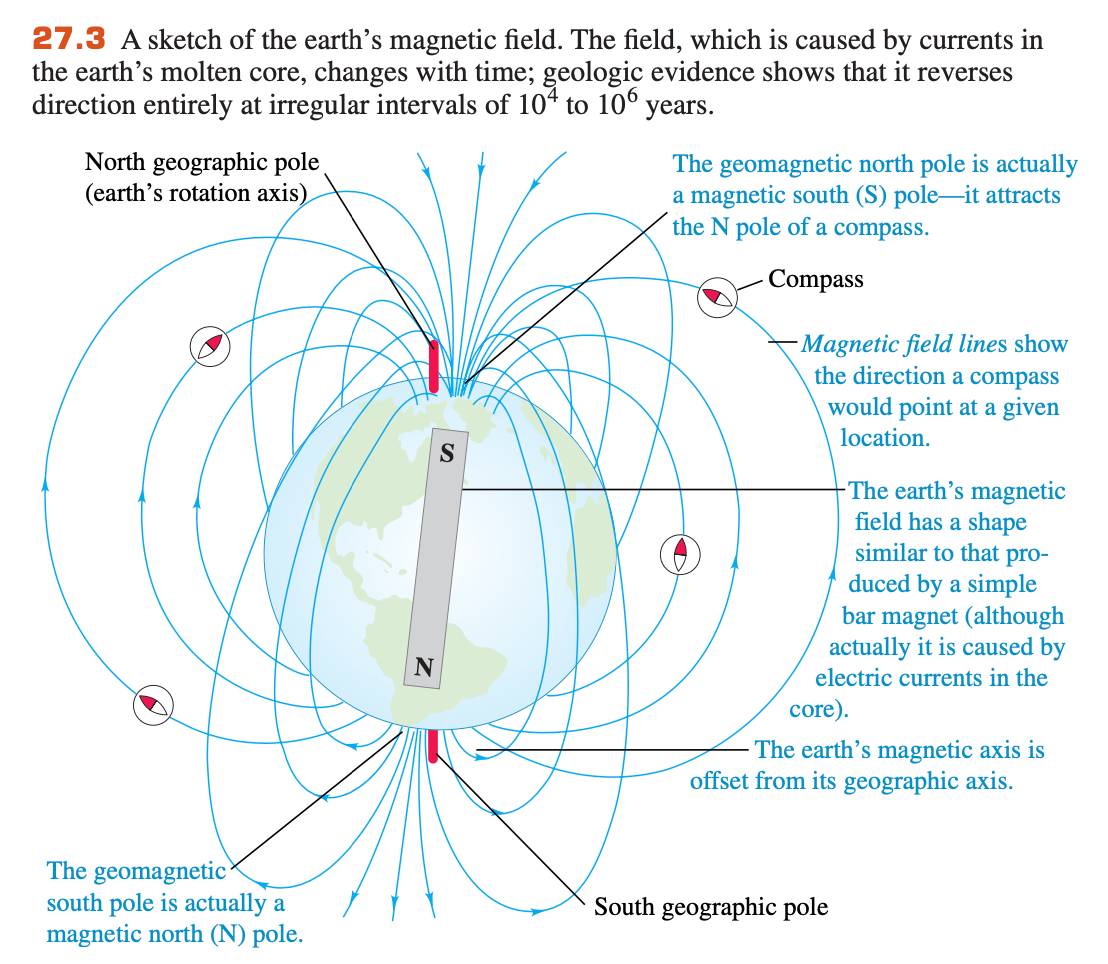
\includegraphics[height = 8cm]{Diagrama1_CampoMagneticoTerrestre.png}
    \caption{Diagrama del campo magnético terrestre}
\end{figure}
Si a una partícula se le da una velocidad inicial, esa partícula siente fuerza debido al campo magnético. No existe fuerza 
magnética si la partícula está estática. Además, éstas partículas no siguen velocidad constante si no que 
se desvían. El campo magnético funciona de manera similar al campo eléctrico: Una corriente o carga en movimiento crea un campo magnético en 
su alrededor, y éste campo ejerce una fuerza sobre cualquier otra carga en movimiento o corriente. Usualmente se usa 
la notación $\vec{B}$ para el campo magnético. \\
Hay 4 características principales de la fuerza magnética: 
\begin{enumerate}
\item La magnitud de la fuerza magnética es proporcional a la magnitud y signo de la carga. (Carga de 2 C experimenta doble de fuerza que carga de 1 C bajo 
el mismo campo magnético). 
\item La magnitud de la fuerza es proporcional a la magnitud del campo magnético. Si duplicas la magnitud, duplicas la fuerza 
que siente una partícula en ese campo. 
\item La fuerza magnética depende de la velocidad de la partícula. Una partícula sin movimiento no siente fuerza magnética. 
\item La fuerza magnética $\vec{F}$ siempre es perpendicular al campo magnético $\vec{B}$ y la velocidad $\vec{v}$. Es decir, la dirección de 
$\vec{F}$ es perpendicular al plano que contiene a $\vec{v}$ y $\vec{B}$. 
\end{enumerate}
Se ha encontrado que la magnitud de la fuerza es proporcional al componente de $\vec{b}$ perpendicular al campo magnético. 
Cuando esa componente es cero (velocidad y campo magnético paralelos o antiparalelos), la fuerza es cero. 
De lo anterior, obtenemos la fórmula que nos da la fuerza (magnitud y dirección) en una carga $q$ con velocidad $\vec{v}$ en un campo magnético:
\begin{align}
\vec{F} = q\vec{v} \times \vec{B} 
\label{eq:eq1}
\intertext{Y para obtener su magnitud}
F = q\ast b\ast Bsin(\phi)
\end{align}
Donde $\phi$ es el ángulo medido en de la dirección de $\vec{v}$ hacia $\vec{B}$. Por lo tanto, la fuerza máxima 
se siente cuando la carga se mueve perpendicular al campo magnético, ya que $\sin(90 \degree) = 1$. Las unidades del campo magnético son 
 $\frac{N}{(Amp)m} = 1 T$ o 1 Tesla. Otra unidad es el Gauss, donde $1G = 10^{-4}T$.\\

\textbf{Regla de la mano derecha}: La regla de la mano derecha dice que para encontrar la dirección de la fuerza que siente una partícula, 
usando la mano derecha se "cierra" en dirección a $\vec{B}$ desde $\vec{v}$ en el plano formado entre éstos dos, y el pulgar nos dirá la 
dirección de la fuerza. Si la carga es negativa, la fuerza irá en dirección contraria que la dada por ésta regla. 
Se muestra a continuación un diagrama explicatorio: 
\begin{figure}[H]
    \centering
    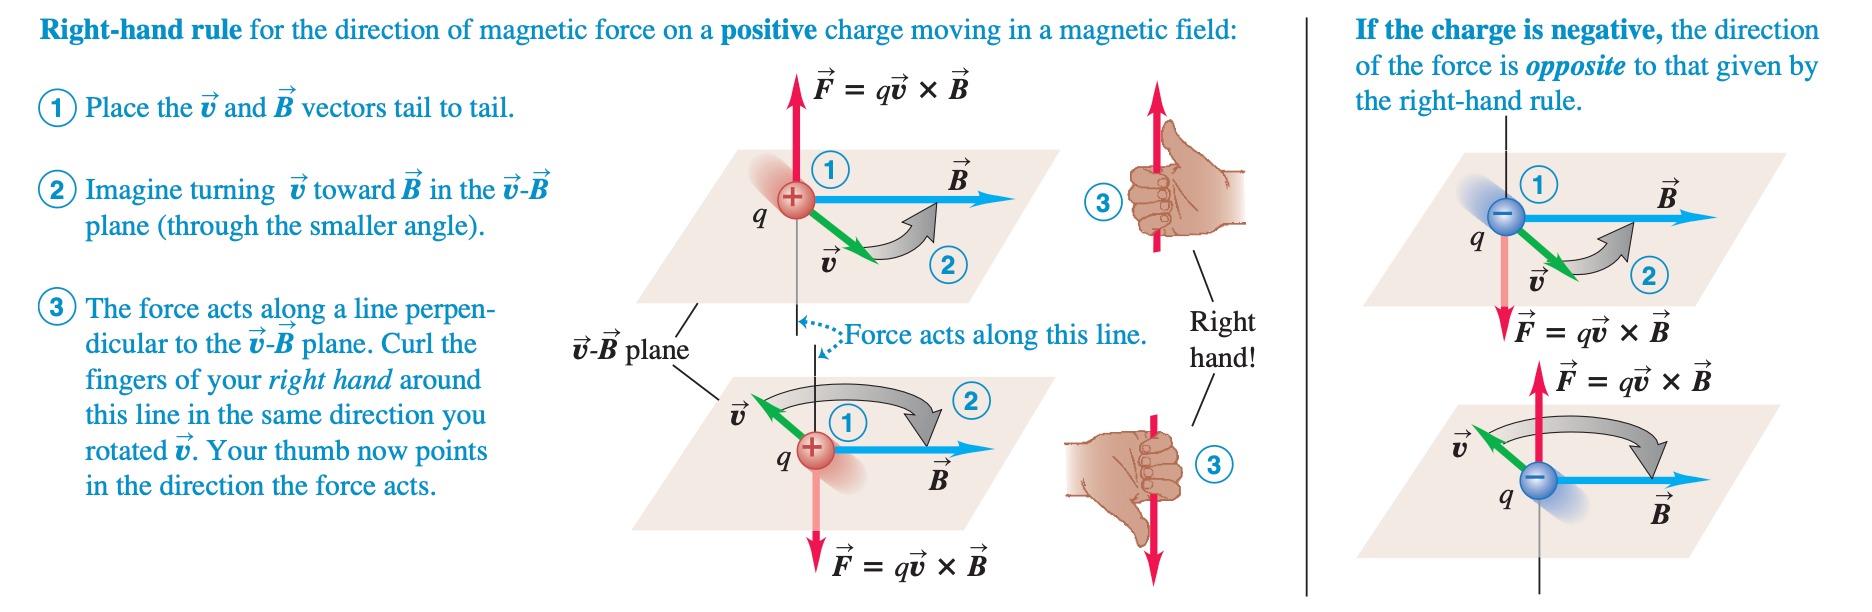
\includegraphics[height = 5cm]{Diagrama2_ReglaManoDerecha_Electromagnetismo.png}
    \caption{Diagrama de la regla de la mano derecha para fuerza magnética}
\end{figure}
Una partícula se mueve en línea recta a velocidad constante cuando $F_b$ y $F_w$ se cancelan, es decir, van en sentidos opuestos 
con la misma magnitud. \\ 

Cuando una partícula se mueve en un campo magnético, la fuerza (magnitud y dirección) nos la da la ecuación \ref{eq:eq1} y su 
movimiento se rige por las leyes de Newton. La fuerza siempre es perpendicular a $vec{v}$, por lo que la fuerza 
no puede cambiar la magnitud de su velocidad, solo su dirección. En otras palabras, como el campo magnético no tiene un 
componente paralelo al movimiento de la partícula, no puede aplicar trabajo en ésta. Entonces, una partícula 
cargada siempre se mueve con velocidad constante dentro de un campo magnético. \\ 

Si observamos el siguiente diagrama: 
\begin{figure}[H]
    \centering
    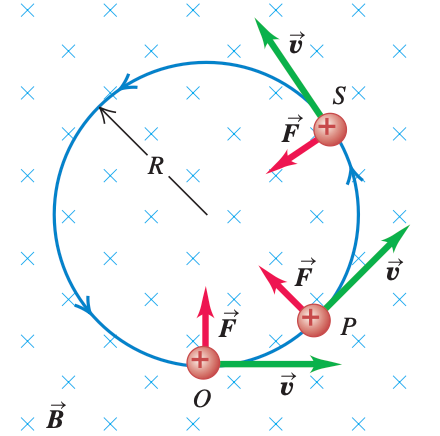
\includegraphics[height = 5cm]{Diagrama3_MovimientoCentripetaCampoMagnetico.png}
    \caption{Movimiento de una partícula en un campo magnético uniforme}
\end{figure}
Podemos ver que las magnitudes de $\vec{F}$ y $\vec{v}$ son constantes es decir su magnitud se mantiene igual. Por lo tanto, 
su aceleración centrípeta es $\frac{v^2}{R}$, y por como solo actúa la fuerza magnética, $F = q\ast v \ast B = m (\frac{V^2}{R})$ siendo $m$ 
la masa de la partícula. De aquí, podemos despejar para $R$ para obtener una fórmula para el radio de una órbita 
circular en un campo magnético: 
\begin{align}
R = \frac{mv}{|q|B}
\label{eq:eq3}
\end{align}
Si la dirección de velocidad inicial no es perpendicular al campo, el componente de la velocidad paralelo al campo es 
constante, y por lo tanto la partícula se mueve en una hélice, el cuál la ecuación \ref{eq:eq3} nos da el radio. 
\end{document}